\documentclass[12pt]{report}
\usepackage[english, magyar]{babel}
\usepackage{t1enc}
\frenchspacing

\usepackage[margin=2cm, top=5cm, bottom=2.5cm, bindingoffset=0cm]{geometry}
\usepackage{graphicx}

\usepackage{hyperref}
\hypersetup{hidelinks}

\usepackage{xcolor,listings}
\usepackage{textcomp}
\usepackage{color}
\usepackage{listingsutf8}

\renewcommand{\lstlistingname}{Programkód}

\definecolor{codegreen}{rgb}{0,0.6,0}
\definecolor{codegray}{rgb}{0.5,0.5,0.5}
\definecolor{codepurple}{HTML}{C42043}
\definecolor{backcolour}{HTML}{F2F2F2}
\definecolor{bookColor}{cmyk}{0,0,0,0.90}  
\definecolor{xmltagcolor}{rgb}{0,0,1}
\definecolor{xmltagcolor}{rgb}{0,0,1}
\definecolor{xmlcommentcolor}{rgb}{0,0.6,0}
\definecolor{xmlstringcolor}{rgb}{0.6,0,0}
\color{bookColor}
\lstset{upquote=true}

\lstdefinestyle{mystyle}{
	language=XML, % Setting the language as XML
	basicstyle=\ttfamily\footnotesize, % Setting the basic style
	morestring=[b]", % Strings are in double quotes
	morestring=[s][\color{xmltagcolor}]{<}{>}, % Coloring XML tags blue
	morecomment=[s][\color{xmlcommentcolor}]{<!--}{-->}, % Coloring comments
	showstringspaces=false, % Not showing spaces in strings
	breaklines=true, % Break long lines
	breakatwhitespace=true, % Break lines at whitespace
	tabsize=2, % Setting tab size
	captionpos=b, % Caption position at bottom
	extendedchars=true, % Allowing extended characters
	keepspaces=true, % Keeping spaces for formatting
}

\lstset{style=mystyle} % Applying the style globally

\usepackage{fancyhdr}
\fancypagestyle{plain}{
\fancyhf{}
\fancyhead[R]{\leftmark}
\fancyhead[L]{\thepage}
\fancyfoot[C]{Adatkezelés XML környezetben}}

\fancyhead[R]{\leftmark}
\fancyhead[L]{\thepage}
\fancyfoot[C]{Adatkezelés XML környezetben}

\begin{document}
	\pagestyle{fancy}
	\title{\Huge JEGYZŐKÖNYV \\ \LARGE Adatkezelés XML környezetben}
	\author{\Large Féléves feladat: Autókereskedés}
	\date{\vspace{250px}
		\begin{flushleft}
			Készítette: \textbf{Szendrei Gábor}\\
			Neptunkód: \textbf{V9ZK10}\\
			Dátum: \textbf{2023. 11. 22.}
		\end{flushleft}
		\vspace{15px}
		\begin{center}
			\textbf{Miskolc, 2023}
		\end{center}}
	\maketitle
	
\tableofcontents
\clearpage

\fancyhf{}
\fancyhead[L]{\thepage}

\chapter{A feladat leírása}
A beadanóm témája egy olyan adatbázis, amely autos cégeket és hozzújuk kapcsolódó egyedeket tartja nyilván.

\begin{itemize}
	\item Autóscég
	\begin{itemize}
		\item ceg\_kod - Elsődleges kulcs
		\item cegnev - Cég nevét tartalmazza
		\item helyrajziSzam - Cég elhelyezkedését tartalmazza
		\item dolgozokSzama - Tárolja a dolgozók számát.
	\end{itemize}
		
	\item Vásárlók
	\begin{itemize}
		\item jog\_kod - Elsődleges kulcs
		\item email\_cim - Vásárló email címe
		\item cim - Összetett tulajdonság (Ország, irányítószám, város, utca/házszám)
		\item Telefonszam - Többértékű tulajdonság
	\end{itemize}

	\item Autós adatok
	\begin{itemize}
		\item forgalmi\_kod - Elsődleges kulcs
		\item ar - Mennyibe kerül az eladásra váró autó
		\item kmOra - Mennyi kilométert tettek már meg az autóval
		\item statusz - Szöveges típus, amibe leírást lehet adni, pl. felújított 
	\end{itemize}

	\item Autós típus
	\begin{itemize}
		\item tipus\_kod - Elsődleges kulcs
		\item gyartasiEv - Mikor gyártották az adott autót
		\item marka - Az autó márkáját tartalmazza
		\item nev - Az autó teljes nevét tartalmazza
	\end{itemize}

	\item Számlázás 
	\begin{itemize}
		\item szamlakod - Elsődleges kulcs
		\item szamlaDatum - Mikor állították ki a számlát
		\item vegosszeg - Adókkal mindennel együtt mennyit fizettek
		\item jogsiszam - A vásárló azonosítására szolgál
	\end{itemize}
\end{itemize}


\chapter{I. feladat - XML/XSD létrehozás}

\section{ER modell}

\begin{figure}[h]
	\centering
	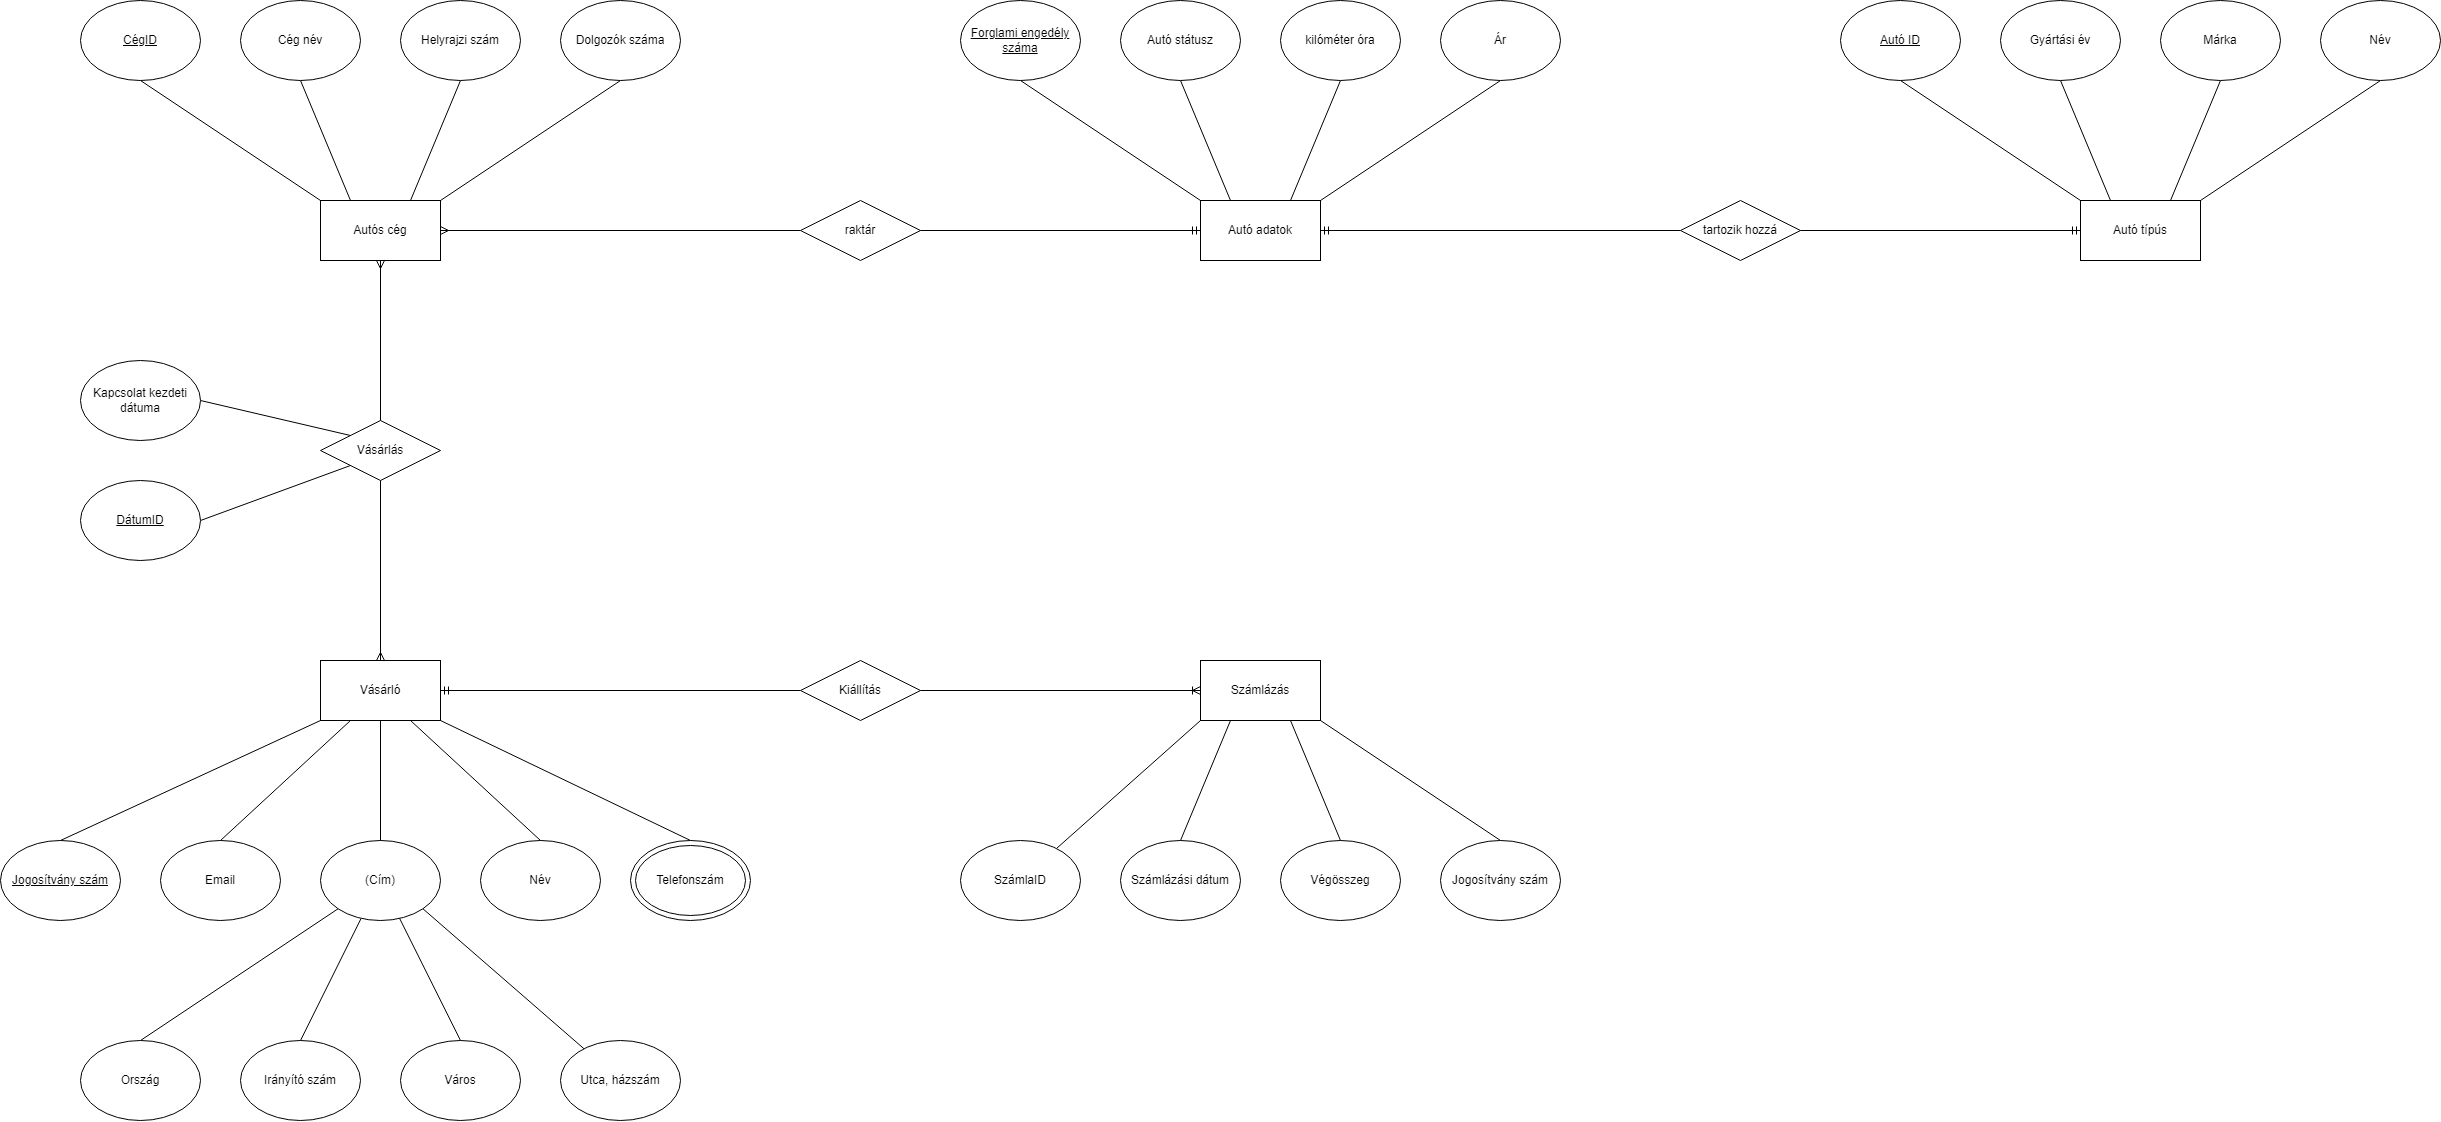
\includegraphics[width=0.999\linewidth]{ERV9ZK10.drawio.png}
	\caption{A feladat ER modellje}
\end{figure}

\begin{itemize}
	\item Autós cég – Autó adatok: 1:n Egy autó több cégnél is megtud fordulni.
	\item Autó adatok – Autó típús 1:1 Egy auto adataihoz egy típús tartozhat csak.
	\item Autós cég – Vásárló n:m  Több vásárló több céghez tartozhat. 
	\item Vásárló – Számlázás Egy vásárlóhoz több számla is tartozhat.
	
\end{itemize}

\section{XDM modell}

XDM modellnél háromféle jelölést alkalmazhatunk. Ezek az ellipszis, a rombusz, illetve a téglalap. Az ellipszis jelöli az elemeket minden egyedből elem lesz, ezen felül a tulajdonságokból is. A rombusz jelöli az attribútumokat, amelyek a kulcs tulajdonságokból keletkeznek. A téglalap jelöli a szöveget, amely majd az XML dokumentumban fog megjelenni. Azoknak az elemeknek, amelyek többször is előfordulhatnak, a jelölése dupla ellipszissel történik. Az idegenkulcsok és a kulcsok közötti kapcsolatot szaggatott vonalas nyíllal jelöljük.
\begin{figure}[h]
	\centering
	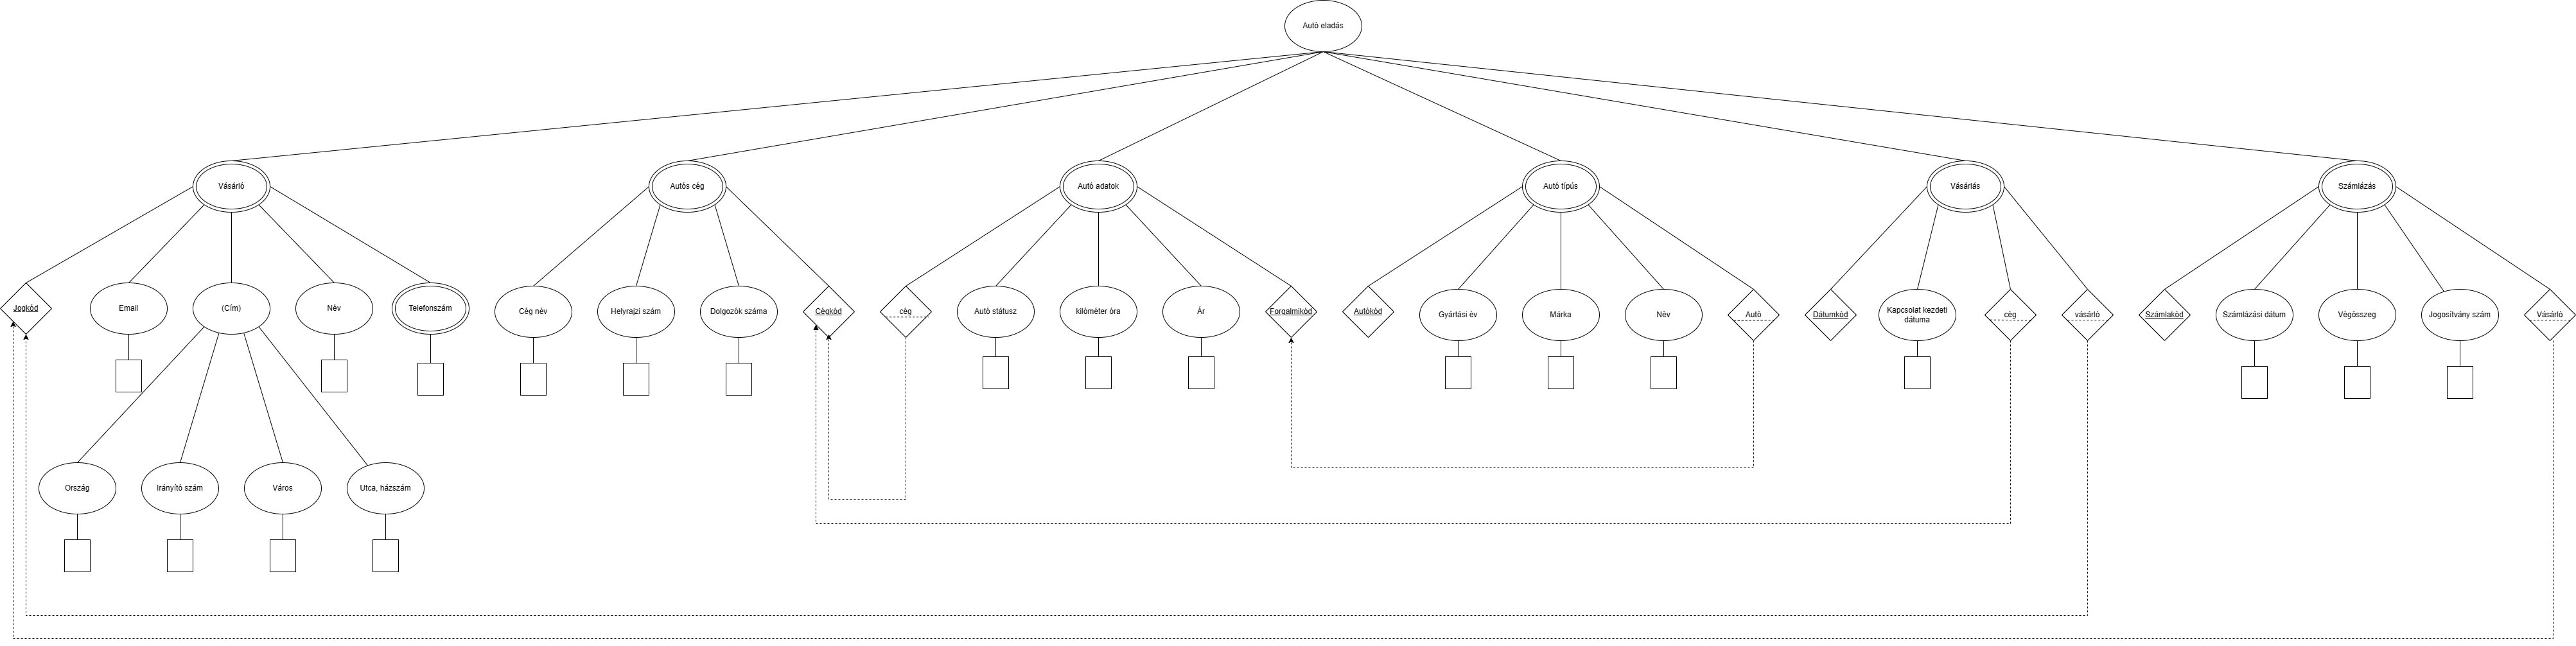
\includegraphics[width=1.01\linewidth]{XDMV9ZK10.drawio.png}
	\caption{A feladat XDM modellje}
\end{figure}

\section[Az XML dokumentum]{Az XDM modell alapján XML dokumentum készítése}
\indent\indent Az \texttt{ERV9ZK10.xml} dokumentumot \textit{Visual Studio Code}-ban hoztam létre, és \texttt{XML 1.0} szabvány szerint készült el. A dokumentumhoz hozzá kötöttem az \texttt{ERV9ZK10.xsd} XSD file-t, és definiáltam az egyedeket az XML szabályainak megfelelően. Ahol szükséges volt, gyermek elemeket, valamint attribútumokat használtam a tagok azonosításához. Az XDM modell alapján az XML dokumentumot úgy készítettem el, hogy először is a gyökér elementtel kezdtem, ami az AutosCegERV9ZK10 volt. A gyermek elemeiből 3-3 példányt hoztam létre, ezeknek az elemeknek az attribútumai közé tartoznak a kulcsok, illetve idegenkulcsok is, mindezek után ezeknek az elemeknek létrehoztam a többi gyermek elementet is.
\begin{lstlisting}[caption={Az XML dokumentum}]
	<?xml version="1.0" encoding="UTF-8"?>
	<AutosCegERV9ZK10 xmlns:xs="http://www.w3.org/2001/XMLSchema-instance"
		xs:noNamespaceSchemaLocation="ERV9ZK10.xsd">
		<Vasarlo jogkod="01">
			<email_cim>jane.smith456@example.com</email_cim>
			<cim>
				<orszag>Magyarorszag</orszag>
				<isz>1234</isz>
				<varos>Budapest</varos>
				<uHsz>Kossuth utca 10</uHsz>
			</cim>
			<nev>Kovacs Peter</nev>
			<Telefonszam>0630-987-6543</Telefonszam>
			<Telefonszam>0630-987-6453</Telefonszam>
		</Vasarlo>
	
		<Vasarlo jogkod="02">
			<email_cim>john.doe456@example.co.uk</email_cim>
			<cim>
				<orszag>Magyarorszag</orszag>
				<isz>5678</isz>
				<varos>Szeged</varos>
				<uHsz>Rakoczi ut 5</uHsz>
			</cim>
			<nev>Nagy Anna</nev>
			<Telefonszam>0620-765-4321</Telefonszam>
			<Telefonszam>0620-765-0000</Telefonszam>
		</Vasarlo>
	
		<Vasarlo jogkod="03">
			<email_cim>mark.johnson789@example.co.uk</email_cim>
			<cim>
				<orszag>Magyarorszag</orszag>
				<isz>9876</isz>
				<varos>Debrecen</varos>
				<uHsz>Petofi ter 3</uHsz>
			</cim>
			<nev>Kiss Eva</nev>
			<Telefonszam>0612-345-6789</Telefonszam>
			<Telefonszam>0630-987-6543</Telefonszam>
		</Vasarlo>
	
		<AutosCeg ceg_kod="11">
			<cegnev>AutaPlusz Kft.</cegnev>
			<helyrajziSzam>BUD-123456</helyrajziSzam>
			<dolgozokSzama>15</dolgozokSzama>
		</AutosCeg>
	
		<AutosCeg ceg_kod="12">
			<cegnev>Autovilag Bt.</cegnev>
			<helyrajziSzam>DEB-654321</helyrajziSzam>
			<dolgozokSzama>10</dolgozokSzama>
		</AutosCeg>
	
		<AutosCeg ceg_kod="13">
			<cegnev>Kocsis Kft.</cegnev>
			<helyrajziSzam>SZEG-987654</helyrajziSzam>
			<dolgozokSzama>20</dolgozokSzama>
		</AutosCeg>
	
		<AutosAdatok forgalmi_kod="21" ceg_kod="11">
			<ar>45000</ar>
			<kmOra>78900</kmOra>
			<statusz>uj</statusz>
		</AutosAdatok>
	
		<AutosAdatok forgalmi_kod="22" ceg_kod="11">
			<ar>55000</ar>
			<kmOra>65400</kmOra>
			<statusz>hasznalt</statusz>
		</AutosAdatok>
	
		<AutosAdatok forgalmi_kod="23" ceg_kod="13">
			<ar>60000</ar>
			<kmOra>89000</kmOra>
			<statusz>hasznalt</statusz>
		</AutosAdatok>
	
		<AutosTipus tipus_kod="31" forgalmi_kod="21">
			<gyartasiEv>2022</gyartasiEv>
			<marka>Toyota</marka>
			<nev>Corolla Hybrid</nev>
		</AutosTipus>
	
		<AutosTipus tipus_kod="32" forgalmi_kod="22">
			<gyartasiEv>2021</gyartasiEv>
			<marka>Volkswagen</marka>
			<nev>Golf GTI</nev>
		</AutosTipus>
	
		<AutosTipus tipus_kod="33" forgalmi_kod="23">
			<gyartasiEv>2020</gyartasiEv>
			<marka>Ford</marka>
			<nev>Focus Titanium</nev>
		</AutosTipus>
	
		<Vasarlas datumkod="41" ceg_kod="11" vasarlo_kod="01">
			<kezdDatum>2023-01-15</kezdDatum>
		</Vasarlas>
	
		<Vasarlas datumkod="42" ceg_kod="12" vasarlo_kod="02">
			<kezdDatum>2023-02-28</kezdDatum>
		</Vasarlas>
	
		<Vasarlas datumkod="43" ceg_kod="13" vasarlo_kod="02">
			<kezdDatum>2023-03-10</kezdDatum>
		</Vasarlas>
	
		<Szamlazas szamlakod="51" vasarlo_kod="01">
			<szamlaDatum>2023-01-20</szamlaDatum>
			<vegosszeg>55000</vegosszeg>
			<jogsiszam>54321</jogsiszam>
		</Szamlazas>
	
		<Szamlazas szamlakod="52" vasarlo_kod="02">
			<szamlaDatum>2023-03-01</szamlaDatum>
			<vegosszeg>60000</vegosszeg>
			<jogsiszam>65432</jogsiszam>
		</Szamlazas>
	
		<Szamlazas szamlakod="53" vasarlo_kod="03">
			<szamlaDatum>2023-04-12</szamlaDatum>
			<vegosszeg>70000</vegosszeg>
			<jogsiszam>76543</jogsiszam>
		</Szamlazas>
	
	</AutosCegERV9ZK10>
\end{lstlisting}
\clearpage

\section{Az XML dokumentum alapján XMLSchema készítése}
\indent\indent Az \texttt{ERV9ZK10.xsd} séma file leírja mindazon megkötéseket, amelyeknek az XML dokumentumnak meg kell felelnie. Itt definiálunk minden típust, amit az XML file-ban használni szeretnénk, valamint az adatbázis kapcsolatait \texttt{xs:unique} és \texttt{xs:keyref} bejegyzésekkel hozom létre. . Az XML Schémám meghatározza az adatokat, mint például a cég nevét, vásárlók címét, telefonszámokat, amelyeket egy \texttt{telefonszamTipus} típus korlátozza, hogy csak bizonyos formátumú (4 szám – 3 szám – 4 szám) fogadja el. Továbbá létezik egy \texttt{emailCimTipus} is, amely szabályozza az emailcím formátumát, amit elfogad. Komplex típusokat is definiáltam, például a \texttt{vasarloTipus}, amiben egy komplex típus definiálja a cím formátumát, \texttt{autosCegTipus}, \texttt{autosAdatokTipus}, \texttt{autosTipusTipus}, \texttt{vasarlasTipus}, \texttt{szamlazasTipus}. Az adatbázis integritásának megőrzése érdekében elsődleges (PK) illetve idegen kulcsok (FK) meghatározására került sor. Az XML séma így biztosítja, hogy az adatok szerkezete és kapcsolatai érvényesek és következetesek legyenek.


\begin{lstlisting}[caption={Az XSD dokumentum}]
	<?xml version="1.0" encoding="UTF-8"?>
	<xs:schema xmlns:xs="http://www.w3.org/2001/XMLSchema">
	
		<!-- Define simple types -->
		<xs:element name="nev" type="xs:string" />
		<xs:element name="cegnev" type="xs:string" />
		<xs:element name="helyrajziSzam" type="xs:string" />
		<xs:element name="dolgozokSzama" type="xs:positiveInteger" />
		<xs:element name="ar" type="xs:positiveInteger" />
		<xs:element name="kmOra" type="xs:positiveInteger" />
		<xs:element name="statusz" type="xs:string" />
		<xs:element name="gyartasiEv" type="xs:positiveInteger" />
		<xs:element name="marka" type="xs:string" />
		<xs:element name="kezdDatum" type="xs:date" />
		<xs:element name="szamlaDatum" type="xs:date" />
		<xs:element name="vegosszeg" type="xs:positiveInteger" />
		<xs:element name="jogsiszam" type="xs:positiveInteger" />
	
		<xs:simpleType name="emailCimTipus">
			<xs:restriction base="xs:string">
				<xs:pattern
					value="([0-9a-zA-Z]([-.\w]*[0-9a-zA-Z])*@([0-9a-zA-Z][-\w]*[0-9a-zA-Z]\.)+[a-zA-Z]{2,9})" />
			</xs:restriction>
		</xs:simpleType>
	
		<xs:simpleType name="telefonszamTipus">
			<xs:restriction base="xs:string">
				<xs:pattern value="\d{4}-\d{3}-\d{4}" />
			</xs:restriction>
		</xs:simpleType>
	
		<!-- Define complex types -->
		<xs:complexType name="vasarloTipus">
			<xs:sequence>
				<xs:element name="email_cim" type="emailCimTipus" />
				<xs:element name="cim">
					<xs:complexType>
						<xs:sequence>
							<xs:element name="orszag" type="xs:string" />
							<xs:element name="isz" type="xs:positiveInteger" />
							<xs:element name="varos" type="xs:string" />
							<xs:element name="uHsz" type="xs:string" />
						</xs:sequence>
					</xs:complexType>
				</xs:element>
				<xs:element ref="nev" />
				<xs:element name="Telefonszam" type="telefonszamTipus" maxOccurs="unbounded" />
			</xs:sequence>
			<xs:attribute name="jogkod" type="xs:integer" use="required" />
		</xs:complexType>
	
		<xs:complexType name="autosCegTipus">
			<xs:sequence>
				<xs:element ref="cegnev" />
				<xs:element ref="helyrajziSzam" />
				<xs:element ref="dolgozokSzama" />
			</xs:sequence>
			<xs:attribute name="ceg_kod" type="xs:integer" use="required" />
		</xs:complexType>
	
		<xs:complexType name="autosAdatokTipus">
			<xs:sequence>
				<xs:element ref="ar" />
				<xs:element ref="kmOra" />
				<xs:element ref="statusz" />
			</xs:sequence>
			<xs:attribute name="forgalmi_kod" type="xs:integer" use="required" />
			<xs:attribute name="ceg_kod" type="xs:integer" use="required" />
		</xs:complexType>
	
		<xs:complexType name="autosTipusTipus">
			<xs:sequence>
				<xs:element ref="gyartasiEv" />
				<xs:element ref="marka" />
				<xs:element ref="nev" />
			</xs:sequence>
			<xs:attribute name="tipus_kod" type="xs:integer" use="required" />
			<xs:attribute name="forgalmi_kod" type="xs:integer" use="required" />
		</xs:complexType>
	
		<xs:complexType name="vasarlasTipus">
			<xs:sequence>
				<xs:element ref="kezdDatum" />
			</xs:sequence>
			<xs:attribute name="datumkod" type="xs:integer" use="required" />
			<xs:attribute name="ceg_kod" type="xs:integer" use="required" />
			<xs:attribute name="vasarlo_kod" type="xs:integer" use="required" />
		</xs:complexType>
	
		<xs:complexType name="szamlazasTipus">
			<xs:sequence>
				<xs:element ref="szamlaDatum"></xs:element>
				<xs:element ref="vegosszeg"></xs:element>
				<xs:element ref="jogsiszam"></xs:element>
			</xs:sequence>
			<xs:attribute name="szamlakod" type="xs:integer" use="required" />
			<xs:attribute name="vasarlo_kod" type="xs:integer" use="required" />
		</xs:complexType>
	
		<!-- Root element with keys and keyrefs -->
		<xs:element name="AutosCegERV9ZK10">
			<xs:complexType>
				<xs:sequence>
					<xs:element name="Vasarlo" type="vasarloTipus" minOccurs="0" maxOccurs="100" />
					<xs:element name="AutosCeg" type="autosCegTipus" minOccurs="0" maxOccurs="100" />
					<xs:element name="AutosAdatok" type="autosAdatokTipus" minOccurs="0"
						maxOccurs="unbounded" />
					<xs:element name="AutosTipus" type="autosTipusTipus" minOccurs="0"
						maxOccurs="unbounded" />
					<xs:element name="Vasarlas" type="vasarlasTipus" minOccurs="0"
						maxOccurs="unbounded" />
					<xs:element name="Szamlazas" type="szamlazasTipus" minOccurs="0"
						maxOccurs="unbounded" />
				</xs:sequence>
			</xs:complexType>
	
			<!-- Primary keys -->
			<xs:key name="vasarlo_kulcs">
				<xs:selector xpath="Vasarlo" />
				<xs:field xpath="@jogkod" />
			</xs:key>
			<xs:key name="AutosCeg_kulcs">
				<xs:selector xpath="AutosCeg" />
				<xs:field xpath="@ceg_kod" />
			</xs:key>
			<xs:key name="AutosAdatok_kulcs">
				<xs:selector xpath="AutosAdatok" />
				<xs:field xpath="@forgalmi_kod" />
			</xs:key>
			<xs:key name="AutosTipus_kulcs">
				<xs:selector xpath="AutosTipus" />
				<xs:field xpath="@tipus_kod" />
			</xs:key>
			<xs:key name="Vasarlas_kulcs">
				<xs:selector xpath="Vasarlas" />
				<xs:field xpath="@datumkod" />
			</xs:key>
			<xs:key name="Szamlazas_kulcs">
				<xs:selector xpath="Szamlazas" />
				<xs:field xpath="@szamlakod" />
			</xs:key>
	
			<!-- Foreign keys -->
			<xs:keyref name="AutosCeg_ceg_kulcs" refer="AutosCeg_kulcs">
				<xs:selector xpath="AutosAdatok" />
				<xs:field xpath="@ceg_kod" />
			</xs:keyref>
			<xs:keyref name="Auto_tipus_AutosAdatok_kulcs" refer="AutosAdatok_kulcs">
				<xs:selector xpath="AutosTipus" />
				<xs:field xpath="@forgalmi_kod" />
			</xs:keyref>
			<xs:keyref name="Vasarlas_ceg_kulcs" refer="AutosCeg_kulcs">
				<xs:selector xpath="Vasarlas" />
				<xs:field xpath="@ceg_kod" />
			</xs:keyref>
			<xs:keyref name="Vasarlas_vasarlo_kulcs" refer="vasarlo_kulcs">
				<xs:selector xpath="Vasarlas" />
				<xs:field xpath="@vasarlo_kod" />
			</xs:keyref>
			<xs:keyref name="Szamlazas_vasarlo_kulcs" refer="vasarlo_kulcs">
				<xs:selector xpath="Szamlazas" />
				<xs:field xpath="@vasarlo_kod" />
			</xs:keyref>
			<!-- Unique constraint for 1:1 relationship -->
			<xs:unique name="AutosAdatok_Auto_tipusok_egyegy">
				<xs:selector xpath="AutosTipus" />
				<xs:field xpath="@forgalmi_kod" />
			</xs:unique>
		</xs:element>
	</xs:schema>
\end{lstlisting}

\chapter{II. feladat - DOM}
\section{Adatolvasás}
\indent\indent A kód egy Java alapú XML feldolgozó program, amely a DOM (Document Object Model) parserét használja. A DOM parser a teljes XML dokumentumot memóriába tölti, ami gyors hozzáférést biztosít az elemekhez, de nagyobb dokumentumok esetén jelentős memóriaigényt jelenthet. A program beolvassa az XML fájlt, normalizálja azt, és különböző függvények segítségével feldolgozza az XML elemeket, melyek az 'Employees', 'Sites', 'Habitats'. Minden elemcsoport feldolgozása külön függvényben történik, ami javítja a kód olvashatóságát és karbantarthatóságát. Hibakezelés is implementálva van a fájlbeolvasás és parse-lás során.\\

\begin{lstlisting}[caption={DOMReadKLNSPG.java} adatolvasó program, language=Java]
	import javax.xml.parsers.*;
	import org.xml.sax.SAXException;
	import org.w3c.dom.*;
	import java.io.*;
	
	public class DOMReadKLNSPG
	{
		// Main metodus
		public static void main(String[] args) 
		{
			try 
			{
				DocumentBuilderFactory factory = DocumentBuilderFactory.newInstance();
				DocumentBuilder builder = factory.newDocumentBuilder();
				Document document = builder.parse(new File("C:\\projects\\KLNSPG_XMLGyak\\XMLTaskKLNSPG\\XMLKLNSPG.xml"));
				
				document.getDocumentElement().normalize();
				System.out.println("<?xml version=\"1.0\" encoding=\"UTF-8\"?>\n");
				System.out.println("<Zoo_KLNSPG xmlns:xsi=\"http://www.w3.org/2001/XMLSchema-instance\" xsi:noNamespaceSchemaLocation=\"XMLSchemaKLNSPG.xsd\">\n");
				
				readEmployees(document);
				readSites(document);
				readHabitats(document);
				readAnimals(document);
				readFoods(document);
				readEats(document);
				readUsers(document);
				
				System.out.println("\n</Zoo_KLNSPG>");
			} 
			catch (ParserConfigurationException | IOException | SAXException e)
			{
				e.printStackTrace();
			}
		}
		
		// Employee Node beolvaso metodus
		private static void readEmployees(Document document) 
		{
			NodeList employeeList = document.getElementsByTagName("Employee");
			for (int temp = 0; temp < employeeList.getLength(); temp++) 
			{
				Node node = employeeList.item(temp);
				if (node.getNodeType() == Node.ELEMENT_NODE) 
				{
					Element eElement = (Element) node;
					String empId = eElement.getAttribute("emp_id");
					String firstName = eElement.getElementsByTagName("first_name").item(0).getTextContent();
					String lastName = eElement.getElementsByTagName("last_name").item(0).getTextContent();
					String birthDate = eElement.getElementsByTagName("birth_date").item(0).getTextContent();
					String sex = eElement.getElementsByTagName("sex").item(0).getTextContent();
					
					System.out.println("    <Employee emp_id=\"" + empId + "\">");
					printElement("first_name", firstName);
					printElement("last_name", lastName);
					printElement("birth_date", birthDate);
					printElement("sex", sex);
					
					// Tobberteku tulajdonsag lekezelese
					if (eElement.getElementsByTagName("posts").getLength() > 0) {
						NodeList posts = eElement.getElementsByTagName("posts").item(0).getChildNodes();
						System.out.println("        <posts>");
						for (int i = 0; i < posts.getLength(); i++) {
							Node postNode = posts.item(i);
							if (postNode.getNodeType() == Node.ELEMENT_NODE) {
								Element postElement = (Element) postNode;
								System.out.println("            <post>" + postElement.getTextContent() + "</post>");
							}
						}
						System.out.println("        </posts>");
					}
					
					System.out.println("    </Employee>");
				}
			}
		}
		
		// Site Node beolvaso metodus
		private static void readSites(Document document) 
		{
			NodeList siteList = document.getElementsByTagName("Site");
			for (int temp = 0; temp < siteList.getLength(); temp++) 
			{
				Node node = siteList.item(temp);
				if (node.getNodeType() == Node.ELEMENT_NODE) 
				{
					Element eElement = (Element) node;
					String siteId = eElement.getAttribute("site_id");
					String works = eElement.getAttribute("Works");
					String manage = eElement.getAttribute("Manage");
					String name = eElement.getElementsByTagName("name").item(0).getTextContent();
					String area = eElement.getElementsByTagName("area").item(0).getTextContent();
					String openingHours = eElement.getElementsByTagName("opening_hours").item(0).getTextContent();
					
					System.out.println("    <Site site_id=\"" + siteId + "\" Works=\"" + works + "\" Manage=\"" + manage + "\">");
					printElement("name", name);
					printElement("area", area);
					printElement("opening_hours", openingHours);
					System.out.println("    </Site>");
				}
			}
		}
		
		// Habitat Node beolvaso metodus
		private static void readHabitats(Document document) 
		{
			NodeList habitatList = document.getElementsByTagName("Habitat");
			for (int temp = 0; temp < habitatList.getLength(); temp++) 
			{
				Node node = habitatList.item(temp);
				if (node.getNodeType() == Node.ELEMENT_NODE) 
				{
					Element eElement = (Element) node;
					String habitatId = eElement.getAttribute("habitat_id");
					String occupy = eElement.getAttribute("Occupy");
					String name = eElement.getElementsByTagName("name").item(0).getTextContent();
					String location = eElement.getElementsByTagName("location").item(0).getTextContent();
					String description = eElement.getElementsByTagName("description").item(0).getTextContent();
					
					System.out.println("    <Habitat habitat_id=\"" + habitatId + "\" Occupy=\"" + occupy + "\">");
					printElement("name", name);
					printElement("location", location);
					printElement("description", description);
					System.out.println("    </Habitat>");
				}
			}
		}
		
		// Animal Node beolvaso metodus
		private static void readAnimals(Document document) 
		{
			NodeList animalList = document.getElementsByTagName("Animal");
			for (int temp = 0; temp < animalList.getLength(); temp++) 
			{
				Node node = animalList.item(temp);
				if (node.getNodeType() == Node.ELEMENT_NODE) 
				{
					Element eElement = (Element) node;
					String animalId = eElement.getAttribute("animal_id");
					String name = eElement.getElementsByTagName("name").item(0).getTextContent();
					String racial = eElement.getElementsByTagName("racial").item(0).getTextContent();
					String description = eElement.getElementsByTagName("description").item(0).getTextContent();
					
					System.out.println("    <Animal animal_id=\"" + animalId + "\">");
					printElement("name", name);
					printElement("racial", racial);
					printElement("description", description);
					System.out.println("    </Animal>");
				}
			}
		}
		
		// Food Node beolvaso metodus
		private static void readFoods(Document document) 
		{
			NodeList foodList = document.getElementsByTagName("Food");
			for (int temp = 0; temp < foodList.getLength(); temp++) 
			{
				Node node = foodList.item(temp);
				if (node.getNodeType() == Node.ELEMENT_NODE) 
				{
					Element eElement = (Element) node;
					String foodId = eElement.getAttribute("food_id");
					String name = eElement.getElementsByTagName("name").item(0).getTextContent();
					String isDelicious = eElement.getElementsByTagName("is_delicious").item(0).getTextContent();
					
					System.out.println("    <Food food_id=\"" + foodId + "\">");
					printElement("name", name);
					printElement("is_delicious", isDelicious);
					
					// Tobberteku tulajdonsag lekezelese
					NodeList companiesNodeList = eElement.getElementsByTagName("companies");
					if (companiesNodeList.getLength() > 0) {
						Node companiesNode = companiesNodeList.item(0);
						if (companiesNode.getNodeType() == Node.ELEMENT_NODE) 
						{
							Element companiesElement = (Element) companiesNode;
							NodeList companyNodeList = companiesElement.getElementsByTagName("company");
							System.out.println("        <companies>");
							for (int i = 0; i < companyNodeList.getLength(); i++) 
							{
								Element companyElement = (Element) companyNodeList.item(i);
								String companyId = companyElement.getAttribute("id");
								System.out.println("            <company id=\"" + companyId + "\">" + companyElement.getTextContent() + "</company>");
							}
							
							System.out.println("        </companies>");
						}
					}
					
					System.out.println("    </Food>");
				}
			}
		}    
		
		// Eat Node beolvaso metodus
		private static void readEats(Document document) 
		{
			NodeList eatList = document.getElementsByTagName("Eat");
			for (int temp = 0; temp < eatList.getLength(); temp++) 
			{
				Node node = eatList.item(temp);
				if (node.getNodeType() == Node.ELEMENT_NODE) 
				{
					Element eElement = (Element) node;
					String eatId = eElement.getAttribute("eat_id");
					String foodEat = eElement.getAttribute("FoodEat");
					String animalEat = eElement.getAttribute("AnimalEat");
					String feedingTime = eElement.getElementsByTagName("feeding_time").item(0).getTextContent();
					
					System.out.println("    <Eat eat_id=\"" + eatId + "\" FoodEat=\"" + foodEat + "\" AnimalEat=\"" + animalEat + "\">");
					printElement("feeding_time", feedingTime);
					System.out.println("    </Eat>");
				}
			}
		}
		
		// User Node beolvaso metodus
		private static void readUsers(Document document)
		{
			NodeList userList = document.getElementsByTagName("User");
			for (int temp = 0; temp < userList.getLength(); temp++) 
			{
				Node node = userList.item(temp);
				if (node.getNodeType() == Node.ELEMENT_NODE) 
				{
					Element eElement = (Element) node;
					String userId = eElement.getAttribute("user_id");
					String favor = eElement.getAttribute("Favor");
					String username = eElement.getElementsByTagName("username").item(0).getTextContent();
					String password = eElement.getElementsByTagName("password").item(0).getTextContent();
					String sex = eElement.getElementsByTagName("sex").item(0).getTextContent();
					String firstName = eElement.getElementsByTagName("first_name").item(0).getTextContent();
					String lastName = eElement.getElementsByTagName("last_name").item(0).getTextContent();
					String postCode = eElement.getElementsByTagName("post_code").item(0).getTextContent();
					String city = eElement.getElementsByTagName("city").item(0).getTextContent();
					String street = eElement.getElementsByTagName("street").item(0).getTextContent();
					String number = eElement.getElementsByTagName("number").item(0).getTextContent();
					
					System.out.println("    <User user_id=\"" + userId + "\" Favor=\"" + favor + "\">");
					printElement("username", username);
					printElement("password", password);
					printElement("sex", sex);
					printElement("first_name", firstName);
					printElement("last_name", lastName);
					printElement("post_code", postCode);
					printElement("city", city);
					printElement("street", street);
					printElement("number", number);
					System.out.println("    </User>");
				}
			}
		}
		
		// Elem kiirato metodus
		private static void printElement(String elementName, String content)
		{
			System.out.println("        <" + elementName + ">" + content + "</" + elementName + ">");
		}
	}
\end{lstlisting}

\section{Adatmódosítás}
\indent\indent Ez a Java program, a DOMModifyKLNSPG, egy XML fájlt olvas be és módosítja azt a DOM (Document Object Model) API segítségével. Az XML fájl, amely egy állatkert adatait tartalmazza, egy előre meghatározott útvonalon található, és a \texttt{DocumentBuilder} osztály segítségével parse-oljuk. A program három fő részre oszlik: \texttt{modifyEmployees}, \texttt{modifySites}, és \texttt{modifyAnimals} metódusokra, melyek különböző XML elemeket módosítanak. Az \texttt{modifyEmployees} metódus az Employee elemek \texttt{emp\_id} attribútumát módosítja, minden \texttt{emp\_id} elé \texttt{,,EMP\_''} előtagot illesztve. A \texttt{modifySites} metódus a Site elemek \texttt{visitor\_capacity} attribútumát állítja be ,,5000''-re, amely a látogatók maximális számát jelenti. A \texttt{modifyAnimals} metódus a \textit{Medve} \texttt{racial} értékkel rendelkező Animal elemek \texttt{description} elemének szövegét módosítja \textbf{,,A medve eros es bator''} szövegre. A módosítások után a program egy \texttt{Transformer} segítségével visszaalakítja és kiírja a módosított DOM-ot XML formátumban. Az XML kiírás során a \texttt{Transformer} beállításai biztosítják a formázott, olvasható kimenetet, az \texttt{OutputKeys.INDENT} beállítás segítségével.\\

\begin{lstlisting}[caption={DOMQModifyKLNSPG.java} adatmódosító program, language=Java]
	import javax.xml.parsers.*;
	import javax.xml.transform.OutputKeys;
	import javax.xml.transform.Transformer;
	import javax.xml.transform.TransformerFactory;
	import javax.xml.transform.dom.DOMSource;
	import javax.xml.transform.stream.StreamResult;
	
	import org.w3c.dom.*;
	import java.io.File;
	
	public class DOMModifyKLNSPG 
	{
		// Main metodus
		public static void main(String argv[])
		{
			try
			{
				File inputFile = new File("C:\\projects\\KLNSPG_XMLGyak\\XMLTaskKLNSPG\\XMLKLNSPG.xml");
				
				DocumentBuilderFactory docFactory = DocumentBuilderFactory.newInstance();
				DocumentBuilder docBuilder = docFactory.newDocumentBuilder();
				Document doc = docBuilder.parse(inputFile);
				
				modifyEmployees(doc);
				modifySites(doc);
				modifyAnimals(doc);
				
				TransformerFactory transformerFactory = TransformerFactory.newInstance();
				Transformer transformer = transformerFactory.newTransformer();
				transformer.setOutputProperty(OutputKeys.INDENT, "yes");
				DOMSource source = new DOMSource(doc);
				StreamResult consoleResult = new StreamResult(System.out);
				transformer.transform(source, consoleResult);
			} 
			catch (Exception e)
			{
				e.printStackTrace();
			}
		}
		
		// Employee peldanyokat modosito metodus
		private static void modifyEmployees(Document doc)
		{
			NodeList employeeList = doc.getElementsByTagName("Employee");
			for (int i = 0; i < employeeList.getLength(); i++)
			{
				Node employee = employeeList.item(i);
				Element eElement = (Element) employee;
				String empId = eElement.getAttribute("emp_id");
				eElement.setAttribute("emp_id", "EMP_" + empId);
			}
		}
		
		// Site peldanyokat modosito metodus
		private static void modifySites(Document doc)
		{
			NodeList siteList = doc.getElementsByTagName("Site");
			for (int i = 0; i < siteList.getLength(); i++)
			{
				Node site = siteList.item(i);
				Element eElement = (Element) site;
				eElement.setAttribute("visitor_capacity", "5000");
			}
		}
		
		// Animal (Medve) peldanyt modosito metodus
		private static void modifyAnimals(Document doc)
		{
			NodeList animalList = doc.getElementsByTagName("Animal");
			for (int i = 0; i < animalList.getLength(); i++)
			{
				Node animal = animalList.item(i);
				Element eElement = (Element) animal;
				if ("Medve".equals(eElement.getElementsByTagName("racial").item(0).getTextContent()))
				eElement.getElementsByTagName("description").item(0).setTextContent("A medve eros es bator");
			}
		}
	}
\end{lstlisting}

\section{Adatlekérdezés}
\indent\indent A program a Java \texttt{DOM Parser}-t használja XML fájlunk feldolgozására, ami lehetővé teszi a XML elemek olvasását és manipulálását egy objektumorientált módon. A kód, az XML fájlt, a \texttt{File} objektumon keresztül tölti be, biztosítva ezzel a fájl elérését és kezelését. A \texttt{DocumentBuilderFactory} és \texttt{DocumentBuilder} osztályok használata a fájl DOM reprezentációjának létrehozásához szükséges, ami egy strukturált, fa-szerű modellt biztosít az XML adatok számára. A program minden egyes lekérdezést egy for ciklus segítségével hajt végre, ahol a \texttt{getElementsByTagName} metódus segítségével specifikus XML elemeket keres. Az elemek feldolgozása során a \texttt{Node} és \texttt{Element} interfészeket használja, amelyek lehetővé teszik az egyes elemek attribútumainak és tartalmának elérését. A lekérdezések eredményét egy \texttt{StringBuilder} objektumba gyűjti, amely hatékonyan kezeli a nagy mennyiségű stringek összefűzését. A kód, az összegyűjtött adatokat XML-szerű formátumban állítja elő.\\

\begin{lstlisting}[caption={DOMQueryKLNSPG.java} adatlekérdező program, language=Java]
import java.io.*;
import javax.xml.parsers.*;
import org.w3c.dom.*;
import org.xml.sax.SAXException;

public class DOMQueryKLNSPG
{
	// Main metodus
	public static void main(String argv[]) throws SAXException, IOException, ParserConfigurationException 
	{
		File xmlFile = new File("C:\\projects\\KLNSPG_XMLGyak\\XMLTaskKLNSPG\\XMLKLNSPG.xml");
		
		DocumentBuilderFactory factory = DocumentBuilderFactory.newInstance();
		DocumentBuilder dBuilder = factory.newDocumentBuilder();
		
		Document doc = dBuilder.parse(xmlFile);
		doc.getDocumentElement().normalize();
		
		StringBuilder outputBuilder = new StringBuilder();
		
		// Lekerdezes a ferfi Employee-kre
		NodeList employeeList = doc.getElementsByTagName("Employee");
		outputBuilder.append("<Employees>\n");
		for (int i = 0; i < employeeList.getLength(); i++) 
		{
			Node node = employeeList.item(i);
			if (node.getNodeType() == Node.ELEMENT_NODE) 
			{
				Element element = (Element) node;
				String sex = element.getElementsByTagName("sex").item(0).getTextContent();
				if (sex.equals("M")) 
				{
					String empId = element.getAttribute("emp_id");
					String firstName = element.getElementsByTagName("first_name").item(0).getTextContent();
					String lastName = element.getElementsByTagName("last_name").item(0).getTextContent();
					String birthDate = element.getElementsByTagName("birth_date").item(0).getTextContent();
					outputBuilder.append(String.format("  <Employee emp_id=\"%s\">\n", empId));
					outputBuilder.append(String.format("    <first_name>%s</first_name>\n", firstName));
					outputBuilder.append(String.format("    <last_name>%s</last_name>\n", lastName));
					outputBuilder.append(String.format("    <birth_date>%s</birth_date>\n", birthDate));
					outputBuilder.append(String.format("    <sex>%s</sex>\n", sex));
					
					// Posts es azok elemeinek kezelese
					NodeList postsList = element.getElementsByTagName("posts");
					if (postsList.getLength() > 0) {
						Node postsNode = postsList.item(0);
						if (postsNode.getNodeType() == Node.ELEMENT_NODE) 
						{
							outputBuilder.append("    <posts>\n");
							NodeList postList = ((Element)postsNode).getElementsByTagName("post");
							for (int j = 0; j < postList.getLength(); j++) 
							{
								Node postNode = postList.item(j);
								if (postNode.getNodeType() == Node.ELEMENT_NODE) 
								{
									String post = postNode.getTextContent();
									outputBuilder.append(String.format("      <post>%s</post>\n", post));
								}
							}
							outputBuilder.append("    </posts>\n");
						}
					}
					
					outputBuilder.append("  </Employee>\n");
				}
			}
		}
		outputBuilder.append("</Employees>\n");
		
		// Lekerdezes a legnagyobb m^3-ru Site-ra
		NodeList siteList = doc.getElementsByTagName("Site");
		int maxArea = 0;
		Element maxAreaElement = null;
		for (int i = 0; i < siteList.getLength(); i++) 
		{
			Node node = siteList.item(i);
			if (node.getNodeType() == Node.ELEMENT_NODE) 
			{
				Element element = (Element) node;
				int currentArea = Integer.parseInt(element.getElementsByTagName("area").item(0).getTextContent());
				if (currentArea > maxArea) 
				{
					maxArea = currentArea;
					maxAreaElement = element;
				}
			}
		}
		if (maxAreaElement != null) 
		{
			String siteId = maxAreaElement.getAttribute("site_id");
			String name = maxAreaElement.getElementsByTagName("name").item(0).getTextContent();
			outputBuilder.append("\n<LargestSite>\n");
			outputBuilder.append(String.format("  <Site ID=\"%s\">\n", siteId));
			outputBuilder.append(String.format("    <Name>%s</Name>\n", name));
			outputBuilder.append(String.format("    <Area>%d</Area>\n", maxArea));
			outputBuilder.append("  </Site>\n");
			outputBuilder.append("</LargestSite>\n");
		}
		
		// Lekerdezes az 1999 utan szuletett Employee-kre
		outputBuilder.append("\n<EmployeesBornAfter1999>\n");
		for (int i = 0; i < employeeList.getLength(); i++) 
		{
			Node node = employeeList.item(i);
			if (node.getNodeType() == Node.ELEMENT_NODE) 
			{
				Element element = (Element) node;
				String birthDate = element.getElementsByTagName("birth_date").item(0).getTextContent();
				int birthYear = Integer.parseInt(birthDate.substring(0, 4));
				if (birthYear > 1999) {
					String empId = element.getAttribute("emp_id");
					String firstName = element.getElementsByTagName("first_name").item(0).getTextContent();
					String lastName = element.getElementsByTagName("last_name").item(0).getTextContent();
					String sex = element.getElementsByTagName("sex").item(0).getTextContent();
					
					outputBuilder.append(String.format("  <Employee emp_id=\"%s\">\n", empId));
					outputBuilder.append(String.format("    <first_name>%s</first_name>\n", firstName));
					outputBuilder.append(String.format("    <last_name>%s</last_name>\n", lastName));
					outputBuilder.append(String.format("    <birth_date>%s</birth_date>\n", birthDate));
					outputBuilder.append(String.format("    <sex>%s</sex>\n", sex));
					
					// Posts es azok elemeinek kezelese
					NodeList postsList = element.getElementsByTagName("posts");
					if (postsList.getLength() > 0) {
						Node postsNode = postsList.item(0);
						if (postsNode.getNodeType() == Node.ELEMENT_NODE) 
						{
							outputBuilder.append("    <posts>\n");
							NodeList postList = ((Element)postsNode).getElementsByTagName("post");
							for (int j = 0; j < postList.getLength(); j++) {
								Node postNode = postList.item(j);
								if (postNode.getNodeType() == Node.ELEMENT_NODE) 
								{
									String post = postNode.getTextContent();
									outputBuilder.append(String.format("      <post>%s</post>\n", post));
								}
							}
							outputBuilder.append("    </posts>\n");
						}
					}
					
					outputBuilder.append("  </Employee>\n");
				}
			}
		}
		outputBuilder.append("</EmployeesBornAfter1999>\n");
		
		// Lekerdezes a "Medve park" nevu Habitat description-jere
		NodeList habitatList = doc.getElementsByTagName("Habitat");
		outputBuilder.append("\n<MedveParkDescription>\n");
		for (int i = 0; i < habitatList.getLength(); i++) 
		{
			Node node = habitatList.item(i);
			if (node.getNodeType() == Node.ELEMENT_NODE) 
			{
				Element element = (Element) node;
				String name = element.getElementsByTagName("name").item(0).getTextContent();
				if (name.equals("Medve park")) 
				{
					String description = element.getElementsByTagName("description").item(0).getTextContent();
					outputBuilder.append(String.format("  <Description>%s</Description>\n", description));
				}
			}
		}
		outputBuilder.append("</MedveParkDescription>\n");
		
		// Lekerdezes a 3. id-ju User lakcimere
		NodeList userList = doc.getElementsByTagName("User");
		outputBuilder.append("\n<UserAddress id=\"3\">\n");
		for (int i = 0; i < userList.getLength(); i++) 
		{
			Node node = userList.item(i);
			if (node.getNodeType() == Node.ELEMENT_NODE) 
			{
				Element element = (Element) node;
				if (element.getAttribute("user_id").equals("3")) 
				{
					String postCode = element.getElementsByTagName("post_code").item(0).getTextContent();
					String city = element.getElementsByTagName("city").item(0).getTextContent();
					String street = element.getElementsByTagName("street").item(0).getTextContent();
					String number = element.getElementsByTagName("number").item(0).getTextContent();
					outputBuilder.append(String.format("  <Address>\n"));
					outputBuilder.append(String.format("    <PostCode>%s</PostCode>\n", postCode));
					outputBuilder.append(String.format("    <City>%s</City>\n", city));
					outputBuilder.append(String.format("    <Street>%s</Street>\n", street));
					outputBuilder.append(String.format("    <Number>%s</Number>\n", number));
					outputBuilder.append("  </Address>\n");
				}
			}
		}
		outputBuilder.append("</UserAddress>\n");
		
		System.out.println(outputBuilder.toString());
	}
}
\end{lstlisting}

\section{Adatírás}
\indent\indent A kód fő funkciója, hogy beolvassa és kiírja az XML tartalmakat a konzolra és fájlba is. A \texttt{main} metódusban az \textit{XMLKLNSPG} fájlt olvassa be a megadott útvonalról, használva a \\ \texttt{DocumentBuilderFactory} és \texttt{DocumentBuilder} osztályokat az XML struktúra elemzéséhez. Ezután normalizálja a dokumentumot a \texttt{normalize} metódussal, ami segít a DOM fa struktúrájának rendezésében.

A kiíratást a \texttt{TransformerFactory} és a \texttt{Transformer} osztályok segítségével végezzük el, pont ahogy az adatmódosító kódban.

A \texttt{writeDocumentToFile} metódus is egy \texttt{Transformer} objektumot használ az XML dokumentum fájlba írásához, tiszteletben tartva az XML formázási szabályokat. Ez a metódus lehetővé teszi egy új XML dokumentumok mentését. A kiírási folyamat során a kód biztosítja az XML szabványoknak megfelelő indentálást és formázást, ami olvashatóbbá és könnyebben értelmezhetővé teszi a kimenetet.

A kivételkezelés a kódban biztosítja, hogy az XML olvasás vagy írás közben fellépő hibák megfelelően kezelve legyenek, megelőzve ezzel a program összeomlását.\\

\begin{lstlisting}[caption={DOMWriteKLNSPG.java} adatíró program, language=Java]
import org.w3c.dom.*;
import org.xml.sax.SAXException;

import javax.xml.parsers.*;
import javax.xml.transform.*;
import javax.xml.transform.dom.DOMSource;
import javax.xml.transform.stream.StreamResult;
import java.io.*;

public class DOMWriteKLNSPG 
{
	public static void main(String[] args) 
	{
		try 
		{
			File inputFile = new File("C:\\projects\\KLNSPG_XMLGyak\\XMLTaskKLNSPG\\XMLKLNSPG.xml");
			DocumentBuilderFactory dbFactory = DocumentBuilderFactory.newInstance();
			DocumentBuilder dBuilder = dbFactory.newDocumentBuilder();
			Document doc = dBuilder.parse(inputFile);
			doc.getDocumentElement().normalize();
			System.out.println("<?xml version=\"1.0\" encoding=\"UTF-8\"?>");
			TransformerFactory transformerFactory = TransformerFactory.newInstance();
			Transformer transformer = transformerFactory.newTransformer();
			transformer.setOutputProperty(OutputKeys.INDENT, "yes");
			DOMSource source = new DOMSource(doc);
			StreamResult consoleResult = new StreamResult(System.out);
			transformer.transform(source, consoleResult);
			writeDocumentToFile(doc, "XMLKLNSPG1.xml");
			
			System.out.println("The content has been written to the output file successfully.");
		} 
		catch (SAXException | IOException | ParserConfigurationException | TransformerException e) 
		{
			e.printStackTrace();
		}
	}
	private static void writeDocumentToFile(Document doc, String filename) throws TransformerException 
	{
		TransformerFactory transformerFactory = TransformerFactory.newInstance();
		Transformer transformer = transformerFactory.newTransformer();
		transformer.setOutputProperty(OutputKeys.INDENT, "yes");
		DOMSource source = new DOMSource(doc);
		StreamResult result = new StreamResult(new File(filename));
		transformer.transform(source, result);
	}
}
\end{lstlisting}

\end{document}